\chapter{Extração e armazenamento de dados de redes sociais para análise de sentimentos}
\label{cha: Extracao}

%\section{Aplicação Math Race  desenvolvido com outras tecnologias}

    No capitulo três foi apresentado cada elemento principal do framework. Neste capítulo será apresentada e analisada, a implementação e funcionamento destes elementos.

Descrição de cada seção comentada.
% Na seção \ref{Comparativo em relação a arquitetura de aplicações LAMP} é apresentado um comparativo entre o MEAN \textit{Stack} e a arquitetura LAMP. A integração das ferramentas do MEAN \textit{Stack} é apresentada na seção \ref{Aplicação Math Race com MEAN Stack}. Na seção \ref{subsec: Testes de desempenho}  são  mostrados os testes realizados em relação ao desempenho.

% A figura \ref{fig:MEAN Stack visto como uma pilha} ilustra a pilha que é formada unindo as tecnologias já explicadas no capítulo anterior. No banco de dados coloca-se o MongoDB, no lado do servidor existe o Node.js e o Express e por último no lado do cliente o AngularJS. A seta de duplo sentido representa que a passagem de dados acontece em ambos os sentidos. O principal motivo para estas tecnologias funcionarem bem em conjunto, é que todas elas têm como base a linguagem Javascript, sendo que esta característica faz parte da proposta do MEAN \textit{Stack} que é o desenvolvimento de aplicações web escaláveis com a utilização de um conjunto de ferramentas em Javascript.

\section{Modelo do banco de dados}
\label{sec: Modelo}
Para fornecer estabilidade e confiabilidade para o armazenamento das informações, escolhemos implementar um banco de dados relacional, já que estas são algumas de suas principais vantagens, como mencionado na seção \ref{sec: BDRelacional}.

\begin{figure}[htb]
\centering
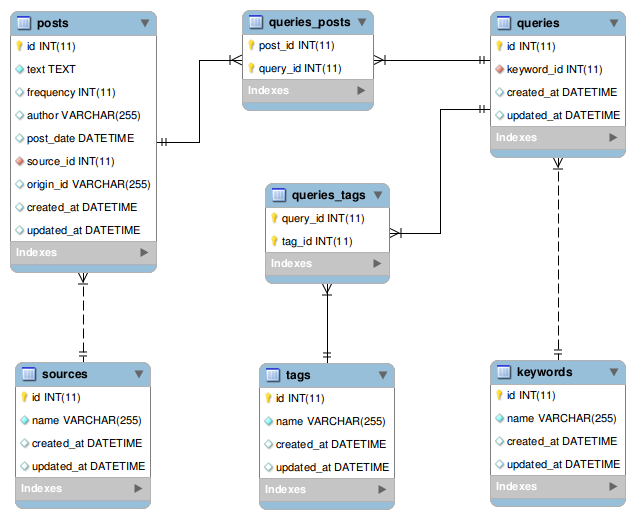
\includegraphics[width=0.8\textwidth]{images/modeloTAZ.png}
\caption{Modelo de entidades e relacionamentos do framework TAZ.}
\label{fig: modeloTAZ}
\end{figure}

Nas subseções seguintes, explicaremos as principais tabelas do modelo \ref{fig: modeloTAZ}, suas colunas mais importantes e as informações que devem ser armazenadas.

\subsection{Palavra-chave (Keywords)}
\label{subsec: Keywords}
Na tabela \textit{keywords} armazenamos as palavras-chave pesquisadas.
\begin{table}[ht]
    \begin{tabular}{|p{3cm}|p{12cm}|}
        \hline
        \rowcolor[HTML]{CFCFCF} 
        Coluna      & Descrição  \\ \hline
        name        & Palavra-chave em si. \\ \hline
    \end{tabular}
    \caption{Descrição dos campos da tabela \textit{keywords}.}
    \label{fig: DescricaoTabelaPalavrasChave}
\end{table}

Uma palavra-chave pode ser utilizada em várias pesquisas.

\subsection{Termos auxiliares (Tags)}
\label{subsec: Tags}
Na tabela \textit{keywords} armazenamos os termos auxiliares usados nas pesquisas realizadas.
\begin{table}[ht]
    \begin{tabular}{|p{3cm}|p{12cm}|}
        \hline
        \rowcolor[HTML]{CFCFCF} 
        Coluna      & Descrição  \\ \hline
        name        & Termo auxiliar. \\ \hline
    \end{tabular}
    \caption{Descrição dos campos da tabela \textit{tags}.}
    \label{fig: DescricaoTabelaTermosAuxiliares}
\end{table}

Um termo auxiliar pode ser usado em várias pesquisas.

\subsection{Pesquisas (Queries)}
\label{subsec: Queries}
Na tabela \textit{queries} são salvos dados de pesquisas. 
\begin{table}[ht]
    \begin{tabular}{|p{3cm}|p{12cm}|}
        \hline
        \rowcolor[HTML]{CFCFCF} 
        Coluna      & Descrição  \\ \hline
        keyword\_id & Identificador da keyword utilizada. \\ \hline
    \end{tabular}
    \caption{Descrição dos campos da tabela \textit{queries}.}
    \label{fig: DescricaoTabelaPesquisas}
\end{table}

Uma pesquisa deve referenciar uma palavra-chave e entre 0 e 3 termos auxiliares.
Também deve estar relacionada a nenhuma ou várias publicações.

\subsection{Fontes (Sources)}
\label{subsec: Sources}
A tabela \textit{sources} contém os nomes das fontes configuradas.
\begin{table}[ht]
    \begin{tabular}{|p{3cm}|p{12cm}|}
        \hline
        \rowcolor[HTML]{CFCFCF} 
        Coluna      & Descrição  \\ \hline
        keyword\_id & Nome da fonte. \\ \hline
    \end{tabular}
    \caption{Descrição dos campos da tabela \textit{sources}.}
    \label{fig: DescricaoTabelaFontes}
\end{table}

Várias publicações podem ser extraídas de uma única fonte.

\subsection{Publicações (Posts)}
\label{subsec: Posts}
Na tabela \textit{posts} são guardadas as publicações das redes sociais.
\begin{table}[ht]
    \begin{tabular}{|p{3cm}|p{12cm}|}
        \hline
        \rowcolor[HTML]{CFCFCF} 
        Coluna      & Descrição  \\ \hline
        text        & Texto da publicação. \\ \hline 
        frequency   & Frequência \footnote{Quantidade de vezes que essa publicação foi reafirmada por outros usuários da rede social. A ação associada à frequência muda para cada rede social e sua representação deve ser especificada pelo desenvolvedor.} que a publicação possui na rede social. \\ \hline 
        author      & Autor da publicação. \\ \hline 
        post\_date  & Data que a publicação foi mandada à rede social. \\ \hline 
        source\_id  & Identificador da fonte cuja a publicação pertence. \\ \hline 
        origin\_id  & Identificador da publicação no banco de dados da rede social . \\ \hline 
    \end{tabular}
    \caption{Descrição dos campos da tabela \textit{posts}.}
    \label{fig: DescricaoTabelaPublicacao}
\end{table}

Uma publicação é extraída somente de uma fonte e pode ser encontrada por várias pesquisas distintas.



\section{Interface}
\label{sec: Interface}

Pensamos em deixar a interface com o usuário a mais simples e intuitiva possível.  Para realizar uma extração basta preencher os campos e opções da página inicial representada na figura \ref{fig: homepage}.

\begin{figure}[htb]
\centering
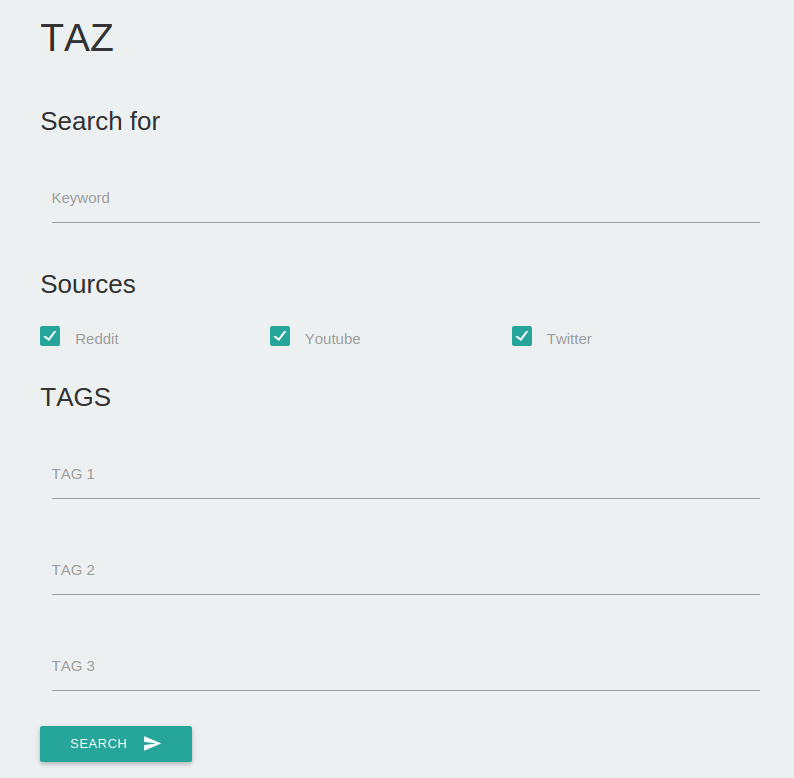
\includegraphics[width=1.0\textwidth]{images/home.png}
\caption{Página inicial do sistema.}
\label{fig: homepage}
\end{figure}

\newpage
A figura \ref{fig: homepage} consiste em:
\begin{enumerate}
    \item Escrever no campo Keyword a palavra pela qual se deseja pesquisar;
    \item Escolher as fontes de extração de informação;
    \item Opcionalmente, adicionar de uma até três Tags. Caso ao menos 1 dos campos Tag seja preenchido, os resultados irão conter no corpo do texto ao menos uma vez os termos especificados pelas Tags;
    \item Clicar no botão Search.
\end{enumerate}

\section{Método de busca}
\label{sec: MetodoDeBusca}
Após preencher o formulário e clicar em Search, o TAZ armazena os valores dos campos do formulário em variáveis locais e monta a string de pesquisa para a API da rede social corrente.

\subsection{Valores dos Campos do Formulário}
\label{subsec: valoresDosCamposDoFormulario}
O critério de pesquisa é definido em duas partes: a keyword (palavra-chave) e as tags ("tradução de tag aqui"). A keyword é o elemento principal para a busca e em combinação com as tags uma a uma, permite uma busca mais específica.

Podemos representar este critério de busca com a seguinte expressão:
$$keyword \wedge (tag1 \vee tag2 \vee tag3)$$

Um exemplo de uso que se adapta ao critério, é a pesquisa da keyword 'Linux', e de duas tags: 'free' e 'code', que será pesquisado pela aplicação textos que tenham as palavras 'linux' e 'free', ou 'linux' e 'code', ou 'linux, 'code' e 'free'.

\subsection{Pesquisa na API}
\label{subsec: PesquisaNaAPI}
No campo source da interface o usuário pode selecionar até três fontes para a busca, que são: Reddit, Youtube e Twitter. Esse campo delimita a origem dos dados a serem retornados na busca, ou seja, dependendo das fontes selecionadas, os métodos das respectivas APIs serão acionados.

\section{Tratamento de resultados}
\label{sec: TratamentoDeResultados}
Caso encontre resultados em pelo menos uma das redes sociais, realiza a análise de sentimentos nos textos obtidos usando o analisador de opiniões textuais SentiWordNet.

O analisador avalia o texto através de uma estimativa de cada palavra. Acessamos o SentiWordNet através de um arquivo de texto que contém uma pontuação de 0.0 à 1.0 para cada palavra quanto a sua positividade e negatividade.
Assim, somando os valores obtidos de cada palavra contida no texto, podemos ter uma ideia da opinião expressa pelo seu autor.

Como nossa aplicação usa vários textos de múltiplas fontes, nós aplicamos uma média ponderada sobre todos os textos, considerando a pontuação do texto obtida do SentiWordNet, e a frequência do texto como peso.

\section{Exibindo estatísticas sobre a análise}
\label{sec: ExibindoEstatisticas}

Com os resultados da análise de sentimento para cada texto de cada publicação, calculamos os seguintes dados estatísticos sobre esta amostra:
\begin{itemize}
    \item Total de textos analisados
    \item Média aritmética simples
    \item Média ponderada considerando a frequência
    \item \textit{maior} nota positiva
    \item \textit{menor} nota positiva
    \item Mediana das notas
    \item Desvio padrão das notas
    \item \% de notas muito positivas (acima de 0.75)
    \item \% de notas positivas (entre 0.25 e 0.75)
    \item \% de notas pouco positivas (entre 0 e 0.25)
    \item \% de notas pouco negativas (entre -0.25 e 0.0)
    \item \% de notas pouco negativas (entre -0.75 e -0.25)
    \item \% de notas pouco negativas (menor que -0.75)
\end{itemize}

!!colocar prints dos gráficos com resultados de \% de textos por faixa.

% Very positive scores are > 0.75
% Positive scores are > 0.25 & <= 0.75
% Weak positive scores are > 0 & <= 0.25
% Weak negative scores are < 0 & >= -0.25
% Negative scores are < -0.25 & >= -0.75
% Very negative scores are < -0.75